\documentclass[twoside]{book}

% Packages required by doxygen
\usepackage{fixltx2e}
\usepackage{calc}
\usepackage{doxygen}
\usepackage[export]{adjustbox} % also loads graphicx
\usepackage{graphicx}
\usepackage[utf8]{inputenc}
\usepackage{makeidx}
\usepackage{multicol}
\usepackage{multirow}
\PassOptionsToPackage{warn}{textcomp}
\usepackage{textcomp}
\usepackage[nointegrals]{wasysym}
\usepackage[table]{xcolor}

% Font selection
\usepackage[T1]{fontenc}
\usepackage[scaled=.90]{helvet}
\usepackage{courier}
\usepackage{amssymb}
\usepackage{sectsty}
\renewcommand{\familydefault}{\sfdefault}
\allsectionsfont{%
  \fontseries{bc}\selectfont%
  \color{darkgray}%
}
\renewcommand{\DoxyLabelFont}{%
  \fontseries{bc}\selectfont%
  \color{darkgray}%
}
\newcommand{\+}{\discretionary{\mbox{\scriptsize$\hookleftarrow$}}{}{}}

% Page & text layout
\usepackage{geometry}
\geometry{%
  a4paper,%
  top=2.5cm,%
  bottom=2.5cm,%
  left=2.5cm,%
  right=2.5cm%
}
\tolerance=750
\hfuzz=15pt
\hbadness=750
\setlength{\emergencystretch}{15pt}
\setlength{\parindent}{0cm}
\setlength{\parskip}{3ex plus 2ex minus 2ex}
\makeatletter
\renewcommand{\paragraph}{%
  \@startsection{paragraph}{4}{0ex}{-1.0ex}{1.0ex}{%
    \normalfont\normalsize\bfseries\SS@parafont%
  }%
}
\renewcommand{\subparagraph}{%
  \@startsection{subparagraph}{5}{0ex}{-1.0ex}{1.0ex}{%
    \normalfont\normalsize\bfseries\SS@subparafont%
  }%
}
\makeatother

% Headers & footers
\usepackage{fancyhdr}
\pagestyle{fancyplain}
\fancyhead[LE]{\fancyplain{}{\bfseries\thepage}}
\fancyhead[CE]{\fancyplain{}{}}
\fancyhead[RE]{\fancyplain{}{\bfseries\leftmark}}
\fancyhead[LO]{\fancyplain{}{\bfseries\rightmark}}
\fancyhead[CO]{\fancyplain{}{}}
\fancyhead[RO]{\fancyplain{}{\bfseries\thepage}}
\fancyfoot[LE]{\fancyplain{}{}}
\fancyfoot[CE]{\fancyplain{}{}}
\fancyfoot[RE]{\fancyplain{}{\bfseries\scriptsize Generated by Doxygen }}
\fancyfoot[LO]{\fancyplain{}{\bfseries\scriptsize Generated by Doxygen }}
\fancyfoot[CO]{\fancyplain{}{}}
\fancyfoot[RO]{\fancyplain{}{}}
\renewcommand{\footrulewidth}{0.4pt}
\renewcommand{\chaptermark}[1]{%
  \markboth{#1}{}%
}
\renewcommand{\sectionmark}[1]{%
  \markright{\thesection\ #1}%
}

% Indices & bibliography
\usepackage{natbib}
\usepackage[titles]{tocloft}
\setcounter{tocdepth}{3}
\setcounter{secnumdepth}{5}
\makeindex

% Hyperlinks (required, but should be loaded last)
\usepackage{ifpdf}
\ifpdf
  \usepackage[pdftex,pagebackref=true]{hyperref}
\else
  \usepackage[ps2pdf,pagebackref=true]{hyperref}
\fi
\hypersetup{%
  colorlinks=true,%
  linkcolor=blue,%
  citecolor=blue,%
  unicode%
}

% Custom commands
\newcommand{\clearemptydoublepage}{%
  \newpage{\pagestyle{empty}\cleardoublepage}%
}

\usepackage{caption}
\captionsetup{labelsep=space,justification=centering,font={bf},singlelinecheck=off,skip=4pt,position=top}

%===== C O N T E N T S =====

\begin{document}

% Titlepage & ToC
\hypersetup{pageanchor=false,
             bookmarksnumbered=true,
             pdfencoding=unicode
            }
\pagenumbering{alph}
\begin{titlepage}
\vspace*{7cm}
\begin{center}%
{\Large Ci\+A402\+Device }\\
\vspace*{1cm}
{\large Generated by Doxygen 1.8.13}\\
\end{center}
\end{titlepage}
\clearemptydoublepage
\pagenumbering{roman}
\tableofcontents
\clearemptydoublepage
\pagenumbering{arabic}
\hypersetup{pageanchor=true}

%--- Begin generated contents ---
\chapter{Ci\+A402\+Device}
\label{md_README}
\Hypertarget{md_README}
Library under CiA 402 standard for device control 
\chapter{Class Index}
\section{Class List}
Here are the classes, structs, unions and interfaces with brief descriptions\+:\begin{DoxyCompactList}
\item\contentsline{section}{\hyperlink{structcan__filter}{can\+\_\+filter} }{\pageref{structcan__filter}}{}
\item\contentsline{section}{\hyperlink{structcan__msg}{can\+\_\+msg} }{\pageref{structcan__msg}}{}
\item\contentsline{section}{\hyperlink{classCanBusPort}{Can\+Bus\+Port} }{\pageref{classCanBusPort}}{}
\item\contentsline{section}{\hyperlink{classCiA301CommPort}{Ci\+A301\+Comm\+Port} }{\pageref{classCiA301CommPort}}{}
\item\contentsline{section}{\hyperlink{classCiA402Device}{Ci\+A402\+Device} }{\pageref{classCiA402Device}}{}
\item\contentsline{section}{\hyperlink{classCiA402DeviceICanbus}{Ci\+A402\+Device\+I\+Canbus} }{\pageref{classCiA402DeviceICanbus}}{}
\item\contentsline{section}{\hyperlink{structco__msg}{co\+\_\+msg} }{\pageref{structco__msg}}{}
\item\contentsline{section}{\hyperlink{classDeviceChain}{Device\+Chain} }{\pageref{classDeviceChain}}{}
\item\contentsline{section}{\hyperlink{structerr__stat}{err\+\_\+stat} }{\pageref{structerr__stat}}{}
\item\contentsline{section}{\hyperlink{classPortBase}{Port\+Base} }{\pageref{classPortBase}}{}
\item\contentsline{section}{\hyperlink{classSocketCanPort}{Socket\+Can\+Port} }{\pageref{classSocketCanPort}}{}
\item\contentsline{section}{\hyperlink{classTestPort}{Test\+Port} }{\pageref{classTestPort}}{}
\end{DoxyCompactList}

\chapter{Class Documentation}
\hypertarget{structcan__filter}{}\section{can\+\_\+filter Struct Reference}
\label{structcan__filter}\index{can\+\_\+filter@{can\+\_\+filter}}
\subsection*{Public Attributes}
\begin{DoxyCompactItemize}
\item 
\mbox{\Hypertarget{structcan__filter_a796cdd0845b3b22c44028a898938d3e0}\label{structcan__filter_a796cdd0845b3b22c44028a898938d3e0}} 
int {\bfseries type}
\item 
\mbox{\Hypertarget{structcan__filter_a4831e5deb6d6475d8cad3ceae529c51f}\label{structcan__filter_a4831e5deb6d6475d8cad3ceae529c51f}} 
\begin{tabbing}
xx\=xx\=xx\=xx\=xx\=xx\=xx\=xx\=xx\=\kill
union \{\\
\>uint32\_t {\bfseries mask}\\
\>uint32\_t {\bfseries upper}\\
\}; \\

\end{tabbing}\item 
\mbox{\Hypertarget{structcan__filter_afbb39bd7340f5fa3ce79d138919840d8}\label{structcan__filter_afbb39bd7340f5fa3ce79d138919840d8}} 
\begin{tabbing}
xx\=xx\=xx\=xx\=xx\=xx\=xx\=xx\=xx\=\kill
union \{\\
\>uint32\_t {\bfseries code}\\
\>uint32\_t {\bfseries lower}\\
\}; \\

\end{tabbing}\end{DoxyCompactItemize}


The documentation for this struct was generated from the following file\+:\begin{DoxyCompactItemize}
\item 
hico\+\_\+api.\+h\end{DoxyCompactItemize}

\hypertarget{structcan__msg}{}\section{can\+\_\+msg Struct Reference}
\label{structcan__msg}\index{can\+\_\+msg@{can\+\_\+msg}}
\subsection*{Public Attributes}
\begin{DoxyCompactItemize}
\item 
\mbox{\Hypertarget{structcan__msg_a233f7f010cc90ec3d453bcb75d66c14e}\label{structcan__msg_a233f7f010cc90ec3d453bcb75d66c14e}} 
\begin{tabbing}
xx\=xx\=xx\=xx\=xx\=xx\=xx\=xx\=xx\=\kill
union \{\\
\>uint16\_t {\bfseries fi}\\
\} {\bfseries PACKED}\\

\end{tabbing}\item 
\mbox{\Hypertarget{structcan__msg_a157aaad2daf039f59606522c6a51663a}\label{structcan__msg_a157aaad2daf039f59606522c6a51663a}} 
uint32\+\_\+t {\bfseries ts}
\item 
\mbox{\Hypertarget{structcan__msg_a9a5f820883d3dfe1f0c6bc33c3f95989}\label{structcan__msg_a9a5f820883d3dfe1f0c6bc33c3f95989}} 
uint32\+\_\+t {\bfseries id}
\item 
\mbox{\Hypertarget{structcan__msg_ac0dab268ebadaa9521b4d535c03f13d8}\label{structcan__msg_ac0dab268ebadaa9521b4d535c03f13d8}} 
uint8\+\_\+t {\bfseries data} \mbox{[}8\mbox{]}
\item 
\mbox{\Hypertarget{structcan__msg_a11a48cac095afd9250fe22fa37929aec}\label{structcan__msg_a11a48cac095afd9250fe22fa37929aec}} 
\begin{tabbing}
xx\=xx\=xx\=xx\=xx\=xx\=xx\=xx\=xx\=\kill
union \{\\
\>uint16\_t {\bfseries fi}\\
\} {\bfseries PACKED}\\

\end{tabbing}\end{DoxyCompactItemize}


The documentation for this struct was generated from the following files\+:\begin{DoxyCompactItemize}
\item 
candatatypes.\+h\item 
hico\+\_\+api.\+h\end{DoxyCompactItemize}

\hypertarget{classCiA402Device}{}\section{Ci\+A402\+Device Class Reference}
\label{classCiA402Device}\index{Ci\+A402\+Device@{Ci\+A402\+Device}}
\subsection*{Public Member Functions}
\begin{DoxyCompactItemize}
\item 
\mbox{\Hypertarget{classCiA402Device_ae71940d1e35a2968a5280bb0f1e5bb5a}\label{classCiA402Device_ae71940d1e35a2968a5280bb0f1e5bb5a}} 
int {\bfseries Check\+Status} ()
\item 
long \hyperlink{classCiA402Device_ab77bce0d7f42429f5f8f092aacb02754}{Switch\+On} ()
\begin{DoxyCompactList}\small\item\em Switch\+On\+: Turn on the device and wait for commands. \end{DoxyCompactList}\item 
long \hyperlink{classCiA402Device_a97acf47b3e3751c85fa70091d3bdfa6a}{Switch\+Off} ()
\begin{DoxyCompactList}\small\item\em Switch\+Off\+: Turn on the device. \end{DoxyCompactList}\item 
double \hyperlink{classCiA402Device_ac8d9e36e6f457565cac7d26d91e4a712}{Get\+Position} ()
\begin{DoxyCompactList}\small\item\em Get\+Position\+: Get the position of the cia 402 device. \end{DoxyCompactList}\end{DoxyCompactItemize}


\subsection{Member Function Documentation}
\mbox{\Hypertarget{classCiA402Device_ac8d9e36e6f457565cac7d26d91e4a712}\label{classCiA402Device_ac8d9e36e6f457565cac7d26d91e4a712}} 
\index{Ci\+A402\+Device@{Ci\+A402\+Device}!Get\+Position@{Get\+Position}}
\index{Get\+Position@{Get\+Position}!Ci\+A402\+Device@{Ci\+A402\+Device}}
\subsubsection{\texorpdfstring{Get\+Position()}{GetPosition()}}
{\footnotesize\ttfamily double Ci\+A402\+Device\+::\+Get\+Position (\begin{DoxyParamCaption}{ }\end{DoxyParamCaption})}



Get\+Position\+: Get the position of the cia 402 device. 

\begin{DoxyReturn}{Returns}
\+: Position (angle in \mbox{[}rad\mbox{]}) 
\end{DoxyReturn}
\mbox{\Hypertarget{classCiA402Device_a97acf47b3e3751c85fa70091d3bdfa6a}\label{classCiA402Device_a97acf47b3e3751c85fa70091d3bdfa6a}} 
\index{Ci\+A402\+Device@{Ci\+A402\+Device}!Switch\+Off@{Switch\+Off}}
\index{Switch\+Off@{Switch\+Off}!Ci\+A402\+Device@{Ci\+A402\+Device}}
\subsubsection{\texorpdfstring{Switch\+Off()}{SwitchOff()}}
{\footnotesize\ttfamily long Ci\+A402\+Device\+::\+Switch\+Off (\begin{DoxyParamCaption}{ }\end{DoxyParamCaption})}



Switch\+Off\+: Turn on the device. 

\begin{DoxyReturn}{Returns}
\+: 0 if correct, negative on errors. 
\end{DoxyReturn}
\mbox{\Hypertarget{classCiA402Device_ab77bce0d7f42429f5f8f092aacb02754}\label{classCiA402Device_ab77bce0d7f42429f5f8f092aacb02754}} 
\index{Ci\+A402\+Device@{Ci\+A402\+Device}!Switch\+On@{Switch\+On}}
\index{Switch\+On@{Switch\+On}!Ci\+A402\+Device@{Ci\+A402\+Device}}
\subsubsection{\texorpdfstring{Switch\+On()}{SwitchOn()}}
{\footnotesize\ttfamily long Ci\+A402\+Device\+::\+Switch\+On (\begin{DoxyParamCaption}{ }\end{DoxyParamCaption})}



Switch\+On\+: Turn on the device and wait for commands. 

\begin{DoxyReturn}{Returns}
\+: 0 if correct, negative on errors. 
\end{DoxyReturn}


The documentation for this class was generated from the following files\+:\begin{DoxyCompactItemize}
\item 
Cia402device.\+h\item 
Cia402device.\+cpp\end{DoxyCompactItemize}

\hypertarget{classCiA402DeviceICanbus}{}\section{Ci\+A402\+Device\+I\+Canbus Class Reference}
\label{classCiA402DeviceICanbus}\index{Ci\+A402\+Device\+I\+Canbus@{Ci\+A402\+Device\+I\+Canbus}}
\subsection*{Public Member Functions}
\begin{DoxyCompactItemize}
\item 
\mbox{\Hypertarget{classCiA402DeviceICanbus_a205b5105bd658b73b582cf1685f1d320}\label{classCiA402DeviceICanbus_a205b5105bd658b73b582cf1685f1d320}} 
{\bfseries Ci\+A402\+Device\+I\+Canbus} (long number, string can\+Port)
\item 
\mbox{\Hypertarget{classCiA402DeviceICanbus_a757447054eadb6824cf779ca58d276ae}\label{classCiA402DeviceICanbus_a757447054eadb6824cf779ca58d276ae}} 
long {\bfseries Init} (const vector$<$ int $>$ \&new\+\_\+can\+Ports, string can\+Port)
\item 
\mbox{\Hypertarget{classCiA402DeviceICanbus_ac831e319febc65d424955e32ecdf72c3}\label{classCiA402DeviceICanbus_ac831e319febc65d424955e32ecdf72c3}} 
int {\bfseries Send\+Message} (\hyperlink{structco__msg}{co\+\_\+msg} input, unsigned int can\+Index)
\item 
\mbox{\Hypertarget{classCiA402DeviceICanbus_aa108188c7f32a1c5d1f50662e66c6676}\label{classCiA402DeviceICanbus_aa108188c7f32a1c5d1f50662e66c6676}} 
long {\bfseries co2c} (const \hyperlink{structco__msg}{co\+\_\+msg} \&input, \hyperlink{structcan__msg}{can\+\_\+msg} \&output)
\item 
\mbox{\Hypertarget{classCiA402DeviceICanbus_a1f8d07b892461470a29ac5d30f3dd679}\label{classCiA402DeviceICanbus_a1f8d07b892461470a29ac5d30f3dd679}} 
int {\bfseries Wait\+For\+Read\+Message} (\hyperlink{structco__msg}{co\+\_\+msg} \&output, unsigned int can\+Index)
\item 
\mbox{\Hypertarget{classCiA402DeviceICanbus_aab504488399b2d5a5a010efef29e3d64}\label{classCiA402DeviceICanbus_aab504488399b2d5a5a010efef29e3d64}} 
long {\bfseries c2co} (const \hyperlink{structcan__msg}{can\+\_\+msg} \&input, \hyperlink{structco__msg}{co\+\_\+msg} \&output)
\item 
\mbox{\Hypertarget{classCiA402DeviceICanbus_aa439b9175f5879282058a3f4c2edb45d}\label{classCiA402DeviceICanbus_aa439b9175f5879282058a3f4c2edb45d}} 
int {\bfseries Set\+Can\+Open\+Msg} (\hyperlink{structco__msg}{co\+\_\+msg} \&msg\+\_\+co)
\item 
\mbox{\Hypertarget{classCiA402DeviceICanbus_af09467b107e73f67804942db1597d983}\label{classCiA402DeviceICanbus_af09467b107e73f67804942db1597d983}} 
int {\bfseries Set\+Can\+Open\+Msg} (\hyperlink{structco__msg}{co\+\_\+msg} \&msg\+\_\+co, uint8\+\_\+t msg\+\_\+start\mbox{[}$\,$\mbox{]})
\item 
\mbox{\Hypertarget{classCiA402DeviceICanbus_a93cde3041c3d0a26666b451aa70b246f}\label{classCiA402DeviceICanbus_a93cde3041c3d0a26666b451aa70b246f}} 
\hyperlink{structcan__msg}{can\+\_\+msg} {\bfseries Set\+Can\+Msg} (\hyperlink{structcan__msg}{can\+\_\+msg} \&msg, uint8\+\_\+t msg\+\_\+start\mbox{[}$\,$\mbox{]})
\item 
\hyperlink{structco__msg}{co\+\_\+msg} \hyperlink{classCiA402DeviceICanbus_ab861fc4d62c917bdb1c06b886c8ed45a}{Set\+Can\+Open\+Msg} (unsigned short id\+\_\+co, unsigned short rtr, vector$<$ uint8\+\_\+t $>$ co\+Data\+Frame)
\begin{DoxyCompactList}\small\item\em Ci\+A402\+Device\+I\+Canbus\+::\+Set\+Can\+Open\+Msg \+: Constructs canopen message from parameters. \end{DoxyCompactList}\end{DoxyCompactItemize}
\subsection*{Public Attributes}
\begin{DoxyCompactItemize}
\item 
\mbox{\Hypertarget{classCiA402DeviceICanbus_a456534a394e4072025f2528938d1070d}\label{classCiA402DeviceICanbus_a456534a394e4072025f2528938d1070d}} 
vector$<$ int $>$ {\bfseries can\+Ports}
\item 
\mbox{\Hypertarget{classCiA402DeviceICanbus_af6cf1493b669ce0415cefed7d84e5710}\label{classCiA402DeviceICanbus_af6cf1493b669ce0415cefed7d84e5710}} 
int {\bfseries ret}
\end{DoxyCompactItemize}


\subsection{Member Function Documentation}
\mbox{\Hypertarget{classCiA402DeviceICanbus_ab861fc4d62c917bdb1c06b886c8ed45a}\label{classCiA402DeviceICanbus_ab861fc4d62c917bdb1c06b886c8ed45a}} 
\index{Ci\+A402\+Device\+I\+Canbus@{Ci\+A402\+Device\+I\+Canbus}!Set\+Can\+Open\+Msg@{Set\+Can\+Open\+Msg}}
\index{Set\+Can\+Open\+Msg@{Set\+Can\+Open\+Msg}!Ci\+A402\+Device\+I\+Canbus@{Ci\+A402\+Device\+I\+Canbus}}
\subsubsection{\texorpdfstring{Set\+Can\+Open\+Msg()}{SetCanOpenMsg()}}
{\footnotesize\ttfamily \hyperlink{structco__msg}{co\+\_\+msg} Ci\+A402\+Device\+I\+Canbus\+::\+Set\+Can\+Open\+Msg (\begin{DoxyParamCaption}\item[{unsigned short}]{id\+\_\+co,  }\item[{unsigned short}]{rtr,  }\item[{vector$<$ uint8\+\_\+t $>$}]{co\+Data\+Frame }\end{DoxyParamCaption})}



Ci\+A402\+Device\+I\+Canbus\+::\+Set\+Can\+Open\+Msg \+: Constructs canopen message from parameters. 


\begin{DoxyParams}{Parameters}
{\em id\+\_\+co} & cob id canopen parameter. \\
\hline
{\em rtr} & request for remote. \\
\hline
{\em msg\+\_\+start} & \+: canopen data frame. \\
\hline
\end{DoxyParams}
\begin{DoxyReturn}{Returns}
\+: canopen constructed message in \hyperlink{structco__msg}{co\+\_\+msg} data type. 
\end{DoxyReturn}


The documentation for this class was generated from the following files\+:\begin{DoxyCompactItemize}
\item 
Ci\+A402\+Device\+I\+Canbus.\+h\item 
Ci\+A402\+Device\+I\+Canbus.\+cpp\end{DoxyCompactItemize}

\hypertarget{structco__msg}{}\section{co\+\_\+msg Struct Reference}
\label{structco__msg}\index{co\+\_\+msg@{co\+\_\+msg}}


{\ttfamily \#include $<$candatatypes.\+h$>$}



Collaboration diagram for co\+\_\+msg\+:\nopagebreak
\begin{figure}[H]
\begin{center}
\leavevmode
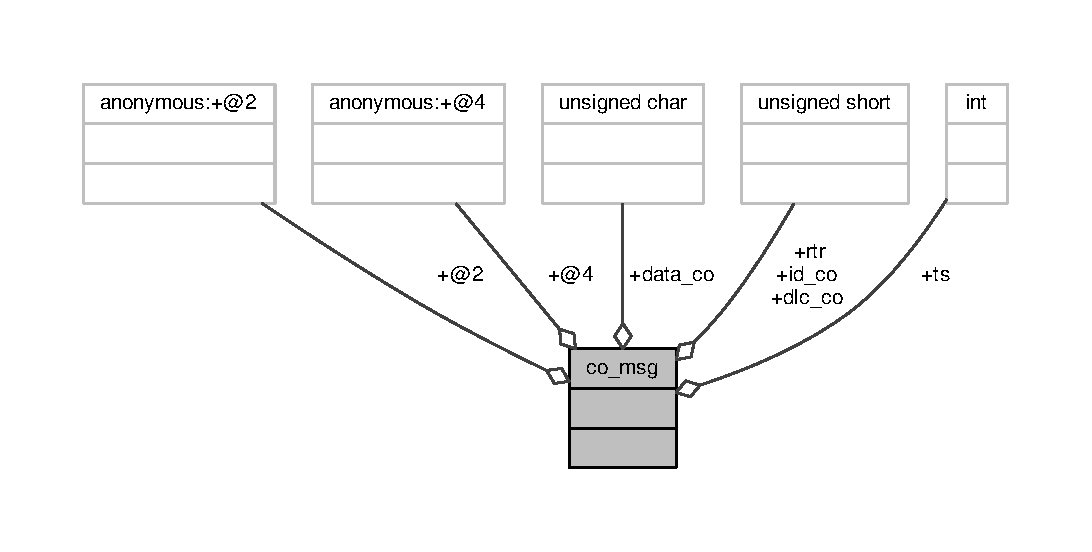
\includegraphics[width=350pt]{structco__msg__coll__graph}
\end{center}
\end{figure}
\subsection*{Public Attributes}
\begin{DoxyCompactItemize}
\item 
\begin{tabbing}
xx\=xx\=xx\=xx\=xx\=xx\=xx\=xx\=xx\=\kill
union \{\\
\>unsigned short \hyperlink{structco__msg_a634de83979d7da90565eccdf16304a07}{id\_co}\\
\}; \\

\end{tabbing}\item 
unsigned int \hyperlink{structco__msg_aaf8cd43d17baf495c982c87866fc90b2}{ts}
\item 
unsigned short \hyperlink{structco__msg_a4352880745fa6bc63d6c4e3c77870029}{rtr}\+:1
\item 
unsigned short \hyperlink{structco__msg_ab19d6996baf97d346427d9789d7e4a6b}{dlc\+\_\+co}
\item 
unsigned char \hyperlink{structco__msg_a3ced1bf4d72ca82fe53c829d42cd946e}{data\+\_\+co} \mbox{[}8\mbox{]}
\item 
\begin{tabbing}
xx\=xx\=xx\=xx\=xx\=xx\=xx\=xx\=xx\=\kill
union \{\\
\>unsigned short \hyperlink{structco__msg_a634de83979d7da90565eccdf16304a07}{id\_co}\\
\}; \\

\end{tabbing}\end{DoxyCompactItemize}


\subsection{Member Data Documentation}
\subsubsection[{\texorpdfstring{"@2}{@2}}]{\setlength{\rightskip}{0pt plus 5cm}union \{ ... \} }\hypertarget{structco__msg_af8251e2eaf9e807267d3ced55e292142}{}\label{structco__msg_af8251e2eaf9e807267d3ced55e292142}
\subsubsection[{\texorpdfstring{"@4}{@4}}]{\setlength{\rightskip}{0pt plus 5cm}union \{ ... \} }\hypertarget{structco__msg_a549464c55b7bbab6345f082dab73b275}{}\label{structco__msg_a549464c55b7bbab6345f082dab73b275}
\index{co\+\_\+msg@{co\+\_\+msg}!data\+\_\+co@{data\+\_\+co}}
\index{data\+\_\+co@{data\+\_\+co}!co\+\_\+msg@{co\+\_\+msg}}
\subsubsection[{\texorpdfstring{data\+\_\+co}{data_co}}]{\setlength{\rightskip}{0pt plus 5cm}unsigned char co\+\_\+msg\+::data\+\_\+co}\hypertarget{structco__msg_a3ced1bf4d72ca82fe53c829d42cd946e}{}\label{structco__msg_a3ced1bf4d72ca82fe53c829d42cd946e}
\index{co\+\_\+msg@{co\+\_\+msg}!dlc\+\_\+co@{dlc\+\_\+co}}
\index{dlc\+\_\+co@{dlc\+\_\+co}!co\+\_\+msg@{co\+\_\+msg}}
\subsubsection[{\texorpdfstring{dlc\+\_\+co}{dlc_co}}]{\setlength{\rightskip}{0pt plus 5cm}unsigned short co\+\_\+msg\+::dlc\+\_\+co}\hypertarget{structco__msg_ab19d6996baf97d346427d9789d7e4a6b}{}\label{structco__msg_ab19d6996baf97d346427d9789d7e4a6b}
\index{co\+\_\+msg@{co\+\_\+msg}!id\+\_\+co@{id\+\_\+co}}
\index{id\+\_\+co@{id\+\_\+co}!co\+\_\+msg@{co\+\_\+msg}}
\subsubsection[{\texorpdfstring{id\+\_\+co}{id_co}}]{\setlength{\rightskip}{0pt plus 5cm}unsigned short co\+\_\+msg\+::id\+\_\+co}\hypertarget{structco__msg_a634de83979d7da90565eccdf16304a07}{}\label{structco__msg_a634de83979d7da90565eccdf16304a07}
\index{co\+\_\+msg@{co\+\_\+msg}!rtr@{rtr}}
\index{rtr@{rtr}!co\+\_\+msg@{co\+\_\+msg}}
\subsubsection[{\texorpdfstring{rtr}{rtr}}]{\setlength{\rightskip}{0pt plus 5cm}unsigned short co\+\_\+msg\+::rtr}\hypertarget{structco__msg_a4352880745fa6bc63d6c4e3c77870029}{}\label{structco__msg_a4352880745fa6bc63d6c4e3c77870029}
\index{co\+\_\+msg@{co\+\_\+msg}!ts@{ts}}
\index{ts@{ts}!co\+\_\+msg@{co\+\_\+msg}}
\subsubsection[{\texorpdfstring{ts}{ts}}]{\setlength{\rightskip}{0pt plus 5cm}unsigned int co\+\_\+msg\+::ts}\hypertarget{structco__msg_aaf8cd43d17baf495c982c87866fc90b2}{}\label{structco__msg_aaf8cd43d17baf495c982c87866fc90b2}


The documentation for this struct was generated from the following files\+:\begin{DoxyCompactItemize}
\item 
\hyperlink{candatatypes_8h}{candatatypes.\+h}\item 
\hyperlink{co__msg_8h}{co\+\_\+msg.\+h}\end{DoxyCompactItemize}

\hypertarget{structerr__stat}{}\section{err\+\_\+stat Struct Reference}
\label{structerr__stat}\index{err\+\_\+stat@{err\+\_\+stat}}


{\ttfamily \#include $<$hico\+\_\+api.\+h$>$}



Collaboration diagram for err\+\_\+stat\+:\nopagebreak
\begin{figure}[H]
\begin{center}
\leavevmode
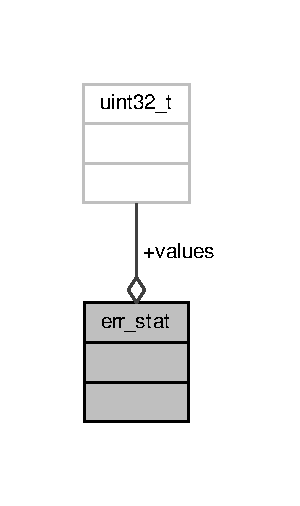
\includegraphics[width=144pt]{structerr__stat__coll__graph}
\end{center}
\end{figure}
\subsection*{Public Attributes}
\begin{DoxyCompactItemize}
\item 
uint32\+\_\+t \hyperlink{structerr__stat_a659e627af5963248da109c8e2404cd08}{values} \mbox{[}0x3f\mbox{]}
\end{DoxyCompactItemize}


\subsection{Member Data Documentation}
\index{err\+\_\+stat@{err\+\_\+stat}!values@{values}}
\index{values@{values}!err\+\_\+stat@{err\+\_\+stat}}
\subsubsection[{\texorpdfstring{values}{values}}]{\setlength{\rightskip}{0pt plus 5cm}uint32\+\_\+t err\+\_\+stat\+::values\mbox{[}0x3f\mbox{]}}\hypertarget{structerr__stat_a659e627af5963248da109c8e2404cd08}{}\label{structerr__stat_a659e627af5963248da109c8e2404cd08}


The documentation for this struct was generated from the following file\+:\begin{DoxyCompactItemize}
\item 
\hyperlink{hico__api_8h}{hico\+\_\+api.\+h}\end{DoxyCompactItemize}

%--- End generated contents ---

% Index
\backmatter
\newpage
\phantomsection
\clearemptydoublepage
\addcontentsline{toc}{chapter}{Index}
\printindex

\end{document}
